\documentclass[czech]{article}% use option titlepage to get the title on a page of its own.
\usepackage{booktabs}
\usepackage{indentfirst}
\usepackage{listings}
\usepackage{hyperref}
\usepackage{fancyhdr}
\usepackage{a4wide}
\usepackage{dblfloatfix}
\usepackage{float}
\usepackage{upgreek}
\usepackage{graphicx}
\usepackage[table,xcdraw]{xcolor}
\usepackage[czech]{babel}
\usepackage[autostyle=true,czech=quotes]{csquotes}

\renewcommand \thesection {\arabic{section}}
\renewcommand \thesubsection {\thesection.\alph{subsection}}
\renewcommand \thesubsubsection {\thesubsection.\alph{subsubsection}}

\title{Pravděpodobnost a statistika\\
    \large Domácí úkoly 1S-4S\\
    \large Zadání 123}

\author{Martin Pustka} 
\date{\today}

\setlength{\headheight}{12.41254pt}
\pagestyle{fancy}
\fancyhf{}
\lhead{Martin Pustka, PUS0065}
\rhead{Číslo zadání 123}
\chead{Ostrava, AR 2020/2021}
\cfoot{\thepage}

\restylefloat{table}
\restylefloat{figure}

\begin{document}

\maketitle

\noindent
Jméno studenta: Martin Pustka\\
Osobní číslo: PUS0065\\
Jméno cvičícího: Ing. Michal Béreš\\

\begin{table*}[!b]
    \centering
    \begin{tabular}{|l|p{5cm}|p{3cm}|}
        \hline
        & Datum odevzdání & Hodnocení \\
        \hline
        Domácí úkol 1: & 9. duben 2021 & 5/5 \\
        \hline
        Domácí úkol 2: & 30. duben 2021 & \\
        \hline
        Domácí úkol 3: & & \\
        \hline
        Domácí úkol 4: & & \\
        \hline
        Celkem: & & \\
        \hline
    \end{tabular}
\end{table*}
\newpage
\tableofcontents
\newpage

\noindent
\textbf{Popis datového souboru}
\\\\
\noindent
Běžné zářivky trpí efektem pomalého nabíhání, tedy plného výkonu dosáhnou až po jisté době provozu. Toto chování je ovlivněno okolní teplotou, což v praxi znamená, že v chladném prostředí může zářivkám trvat výrazně déle než dosáhnou maximálního výkonu. 
\\\\
\noindent
Pro test náběhu zářivek na plný světelný výkon bylo vybráno celkem 350 zářivek od čtyř různých výrobců (Amber, Bright, Clear, Dim). Všechny zářivky měly deklarovaný maximální světelný tok 1000 lm. U každé zářivky byl změřen světelný tok po 30 sekundách od zapnutí, nejprve při teplotě 22 °C a poté při teplotě 5°C.
\\\\
\noindent
V souboru ukol\_X.xslx jsou pro každou z testovaných zářivek uvedeny následující údaje:
\begin{itemize}
    \item pořadové číslo zářivky,
    \item výrobce – Amber (A), Bright (B), Clear (C), Dim (D),
    \item naměřený světelný tok v lumenech při okolní teplotě 5°C,
    \item naměřený světelný tok v lumenech při okolní teplotě 22°C.
\end{itemize}

\noindent
\textbf{Obecné pokyny:}
\begin{itemize}
    \item Úkoly zpracujte dle obecně známých typografických pravidel.
    \item Všechny tabulky i obrázky musí být opatřeny titulkem.
    \item Do úkolů nevkládejte tabulky a obrázky, na něž se v doprovodném textu nebudete odkazovat.
    \item Bude-li to potřeba, citujte zdroje dle mezinárodně platné citační normy ČSN ISO 690.
\end{itemize}


\newpage
\section{Úkol 1S}
\subsection{Zadání}
Pomocí nástrojů explorační analýzy analyzujte světelný tok zářivek výrobce Amber po 30 sekundách od zapnutí při teplotách 5°C a 22°C. Data vhodně graficky prezentujte (krabicový graf, histogram, q-q graf) a doplňte následující tabulky a text.

Výsledky popisné statistiky lze vidět v tabulce \ref{tab:statAmber} a na obrazcích \ref{fig:Boxploty},\ref{fig:Histogram5},\ref{fig:Histogram22},\ref{fig:QQ5} a \ref{fig:QQ22}.
Boxplot obsahuje odlehlá pozorování, ostatní grafy jsou bez odlehlých pozorování.

\subsection{Tabulkové řešení}
\noindent
\begin{table}[H]
	\centering
	\caption{Světelný tok (lm) zářivek Amber v závislosti na teplotě (souhrnné statistiky)}
	\label{tab:statAmber}
	\begin{tabular}{lccl|cc}
        \hline
        \rowcolor[HTML]{F2F2F2} 
        \multicolumn{2}{l}{\cellcolor[HTML]{F2F2F2}Světelný tok zářivek Amber (lm)} & & & \multicolumn{2}{l}{\cellcolor[HTML]{F2F2F2}Po   odstranění odlehlých pozorování} \\
        \rowcolor[HTML]{F2F2F2} 
        \hline
        & 5°C             & 22°C             && 5°C                                    & 22°C                                    \\
        \hline
        rozsah souboru           & 71                          & 71                           &  & 70                                     & 71                                   \\
        minimum                  & 750,0                       & 755,8                        &  & 750,0                                  & 755,8                                   \\
        dolní kvartil            & 774,0                       & 774,0                        &  & 773,4                                  & 774,0                                   \\
        medián                   & 797,8                       & 801,9                        &  & 797,4                                  & 801,9                                   \\
        průměr                   & 797,5                       & 797,6                        &  & 795,6                                  & 797,6                                   \\
        horní kvartil            & 818,3                       & 819,6                        &  & 817,9                                  & 819,6                                   \\
        maximum                  & 927,4                       & 875,1                        &  & 882,9                                  & 875,1                                   \\
        směrodatná odchylka      & 30,5                        & 25,8                         &  & 26,4                                   & 25,8                                    \\
        variační koeficient (\%) & 3,8                         & 3,2                          &  & 3,3                                    & 3,2                                     \\
        šikmost                  & 1,2                         & 0,1                          &  & 0,3                                    & 0,1                                     \\
        špičatost                & 3,4                         & -0,5                         &  & 0,0                                    & -0,5                                    \\
        \hline
        \rowcolor[HTML]{F2F2F2} 
        \multicolumn{3}{l}{\cellcolor[HTML]{F2F2F2}Identifikace   odlehlých pozorování – vnitřní hradby}                 &&   &                                         \\
        \hline
        dolní mez                & 707,6                       & 705,6                        &  & 706,6                                  & 705,6                                   \\
        horní mez                & 884,7                       & 888,0                        &  & 884,6                                  & 888,0                                   \\
        \hline
    \end{tabular}
\end{table}

\newpage
\subsection{Grafické řešení}

\begin{figure}[H]
	\centering
	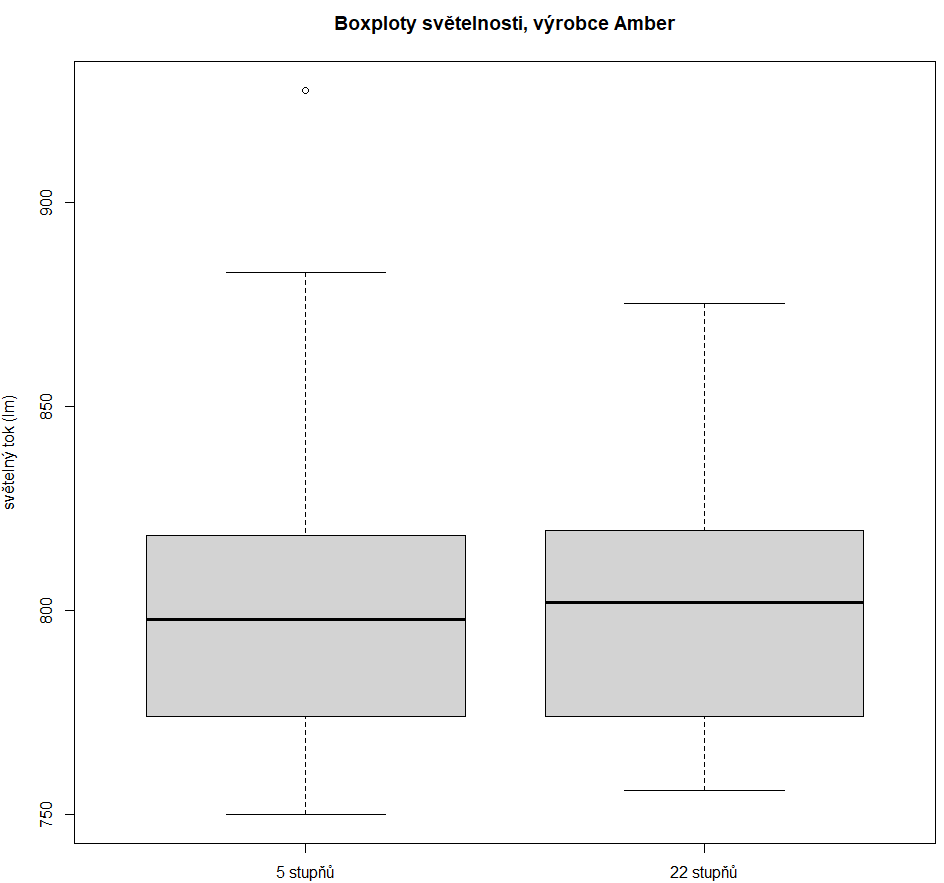
\includegraphics[width=0.6\textwidth]{Figures/Boxploty.png}
	\caption[Boxploty světelnosti, Amber]{Boxploty světelnosti, Amber}
	\label{fig:Boxploty}
\end{figure}

\newpage
\begin{figure}[H]
	\centering
	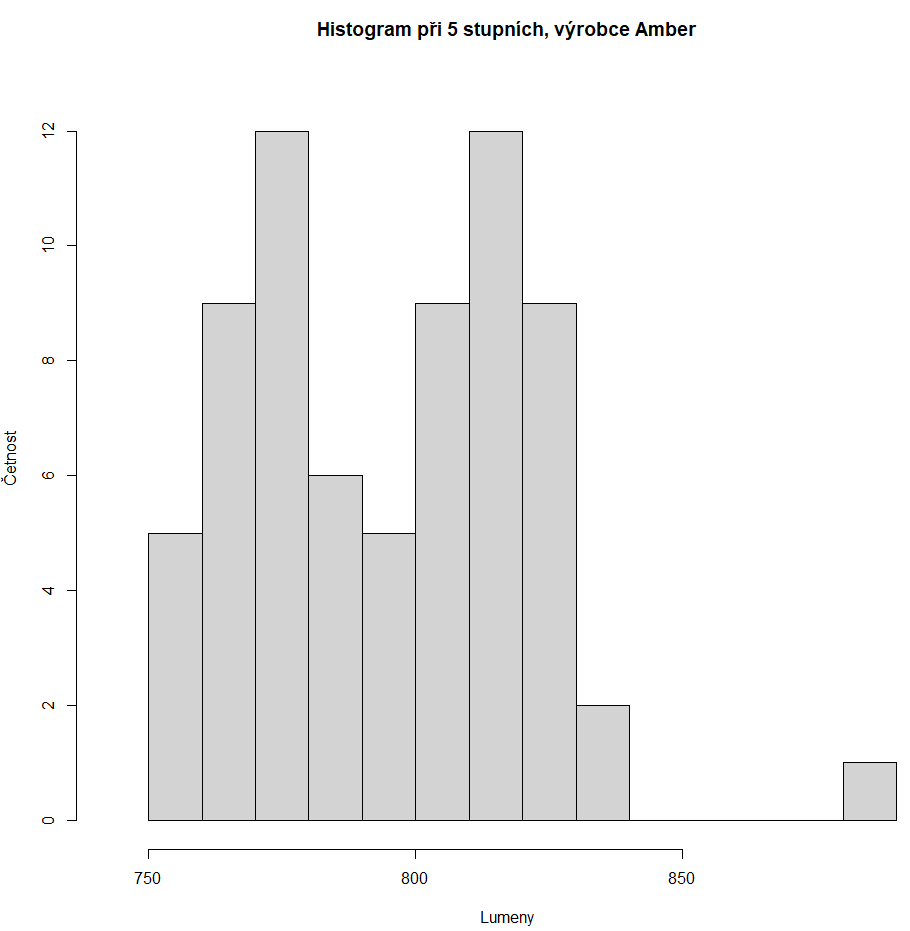
\includegraphics[width=0.6\textwidth]{Figures/Histogram5.png}
	\caption[Histogram světelnosti 5C, Amber]{Histogram světelnosti při 5 stupních, výrobce Amber}
	\label{fig:Histogram5}
\end{figure}

\begin{figure}[H]
	\centering
	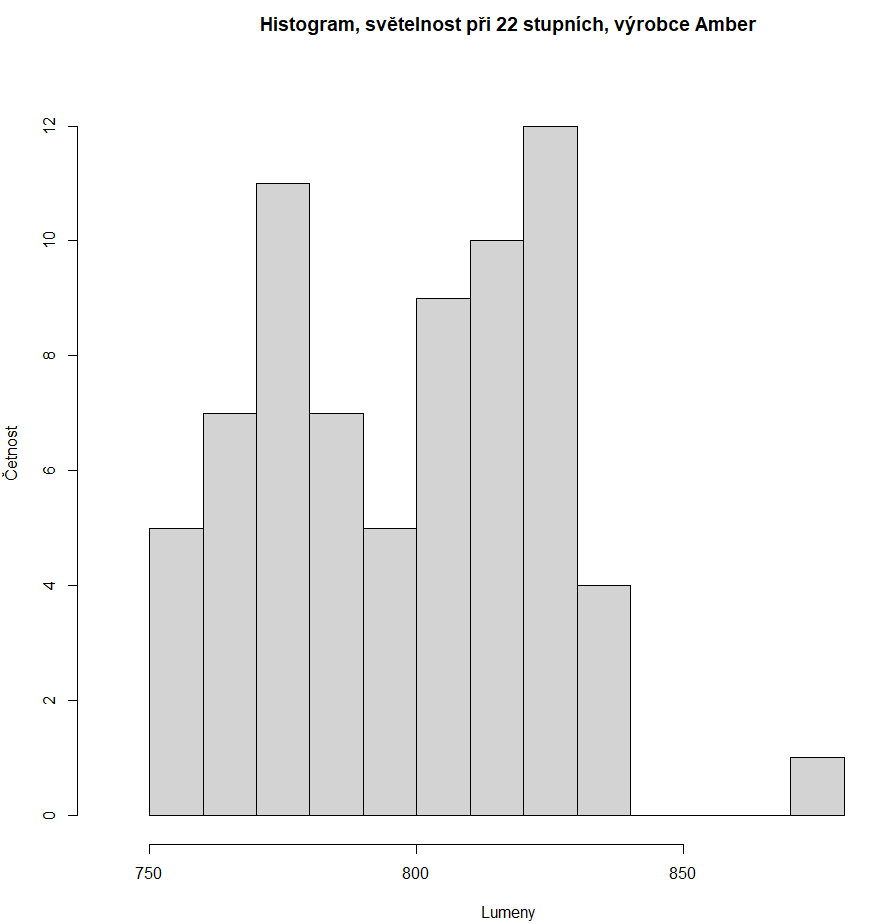
\includegraphics[width=0.6\textwidth]{Figures/Histogram22.png}
	\caption[Histogram světelnosti 22C, Amber]{Histogram světelnosti při 22 stupních, výrobce Amber}
	\label{fig:Histogram22}
\end{figure}

\newpage
\begin{figure}[H]
	\centering
	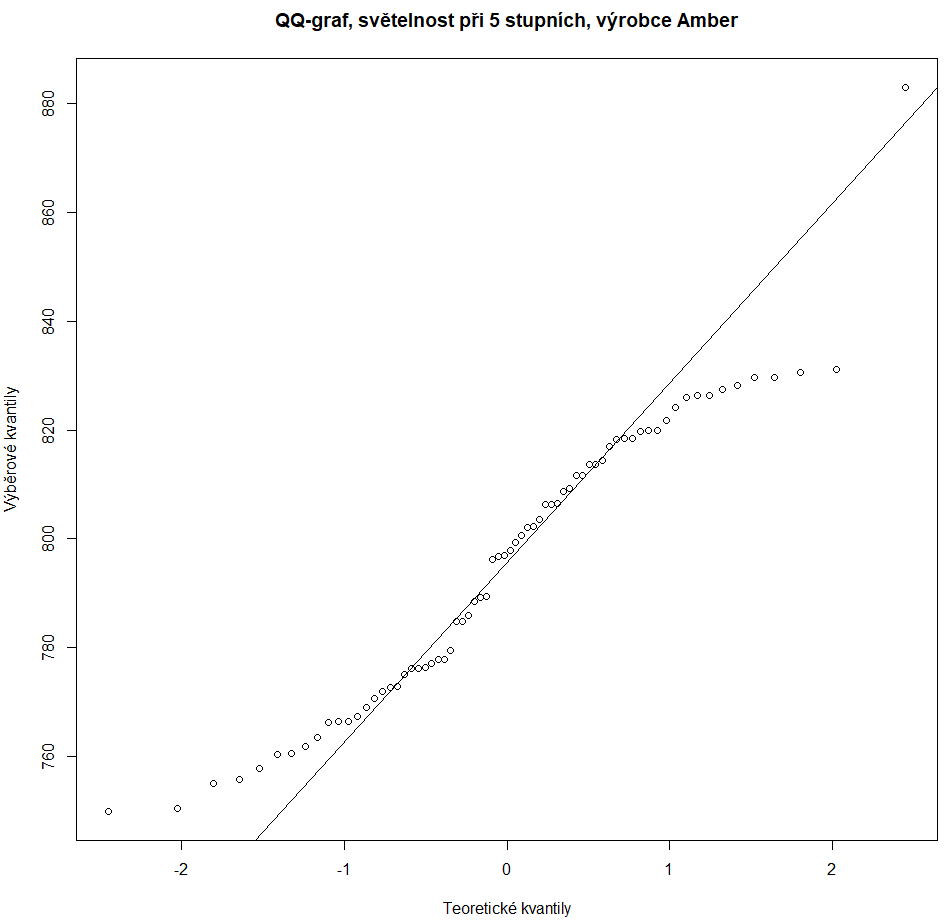
\includegraphics[width=0.6\textwidth]{Figures/QQ5.png}
	\caption[QQ graf světelnosti 5C, Amber]{QQ graf světelnosti při 5 stupních, výrobce Amber}
	\label{fig:QQ5}
\end{figure}

\begin{figure}[H]
	\centering
	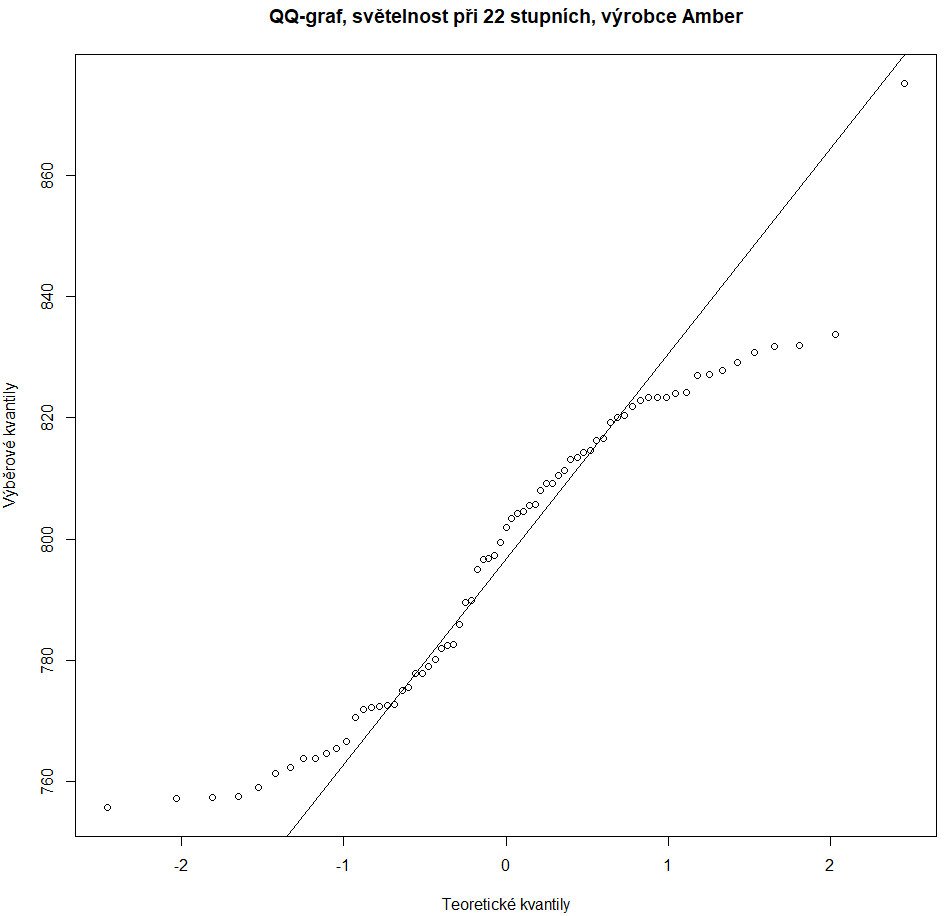
\includegraphics[width=0.6\textwidth]{Figures/QQ22.png}
	\caption[QQ graf světelnosti 5C, Amber]{QQ graf světelnosti při 5 stupních, výrobce Amber}
	\label{fig:QQ22}
\end{figure}

\newpage
\subsection{Textové řešení}

\textbf{Analýza světelného toku zářivek výrobce Amber (po 30 sekundách od zapnutí, při teplotě 5°C)}

Během testu byl měřen světelný tok \textit{71} kusů zářivek výrobce Amber. 
Naměřená světelný tok při teplotě 5°C se pohyboval v rozmezí \textit{750,0} lm až \textit{927,4} lm. 
Světelný tok zářivek č. \textit{27} byl na základě metody vnitřních hradeb identifikován jako 
odlehlé pozorování a nebude zahrnut do dalšího zpracování. Možné příčiny vzniku odlehlých pozorování jsou: \textit{chyby v měření nebo při výrobě}. 
Dále uvedené výsledky tedy pocházejí z analýzy světelný toku \textit{70} kusů zářivek. Jejich průměrný světelný tok byl \textit{795,6} lm, 
směrodatná odchylka pak \textit{26,4} lm. U poloviny testovaných zářivek světelný tok nepřekročil \textit{797,4} lm. 
V polovině měření se světelný tok pohyboval v rozmezí \textit{773,4} lm až \textit{817,9} lm. 
Vzhledem k hodnotě variačního koeficientu (\textit{3,3 \%}) lze analyzovaný soubor považovat za homogenní.\\


\textbf{Analýza světelného toku zářivek výrobce Amber (po 30 sekundách od zapnutí, při teplotě 22°C)}

Během testu byl měřen světelný tok \textit{71} kusů zářivek výrobce Amber. 
Naměřená světelný tok při teplotě 22°C se pohyboval v rozmezí \textit{755,8} lm až \textit{875,1} lm. 
Žádné z měření nebylo identifikováno jako odlehlé pozorování. 
Dále uvedené výsledky tedy pocházejí z analýzy světelný toku \textit{71} kusů zářivek. Jejich průměrný světelný tok byl \textit{797,6} lm, 
směrodatná odchylka pak \textit{25,8} lm. U poloviny testovaných zářivek světelný tok nepřekročil \textit{801,9} lm. 
V polovině měření se světelný tok pohyboval v rozmezí  \textit{774,0} lm až \textit{819,6} lm. 
Vzhledem k hodnotě variačního koeficientu (\textit{3,2} \%) lze analyzovaný soubor považovat za homogenní.\\


\textbf{Ověření normality světelného toku zářivek výrobce Amber po 30 sekundách od zapnutí při teplotě 5°C na základě explorační analýzy}

Na základě grafického zobrazení (viz obrázek \ref{fig:QQ5}) a výběrové šikmosti a špičatosti (výběrová šikmost i špičatost leží v intervalu (-2;2)) 
lze předpokládat, že světelný tok zářivek výrobce Amber při teplotě 5°C má normální rozdělení. Dle pravidla 3$\upsigma$ 
lze tedy očekávat, že přibližně 95 \% zářivek bude mít světelný tok v rozmezí \textit{742,9} lm až \textit{848,3} lm.\\


\textbf{Ověření normality světelného toku zářivek výrobce Amber po 30 sekundách od zapnutí při teplotě 22°C na základě explorační analýzy}

Na základě grafického zobrazení (viz obrázek \ref{fig:QQ22}) a výběrové šikmosti a špičatosti (výběrová šikmost i špičatost leží v intervalu (-2;2)) 
lze předpokládat, že světelný tok zářivek výrobce Amber při teplotě 22°C má normální rozdělení. Dle pravidla 3$\upsigma$ 
lze tedy očekávat, že přibližně 95 \% zářivek bude mít světelný tok v rozmezí \textit{746,0} lm až \textit{849,2} lm.\\


\newpage
\section{Úkol 2S}
Porovnejte pokles světelného toku po 30 sekundách od zapnutí při snížení okolní teploty z 22°C 
na 5°C u zářivek od výrobců Amber a Bright. Nezapomeňte, že použité metody mohou vyžadovat 
splnění určitých předpokladů. Pokud tomu tak bude, okomentujte splnění/nesplnění těchto předpokladů 
jak na základě explorační analýzy (např. s odkazem na histogram apod.), tak exaktně pomocí metod statistické indukce.


\subsection{}
Graficky prezentujte srovnání poklesů světelného toku zářivek výrobců Amber a Bright 
při snížení okolní teploty (vícenásobný krabicový graf, histogramy, q-q grafy). 
Srovnání okomentujte (včetně informace o případné manipulaci sdatovým souborem).

\begin{figure}[H]
	\centering
	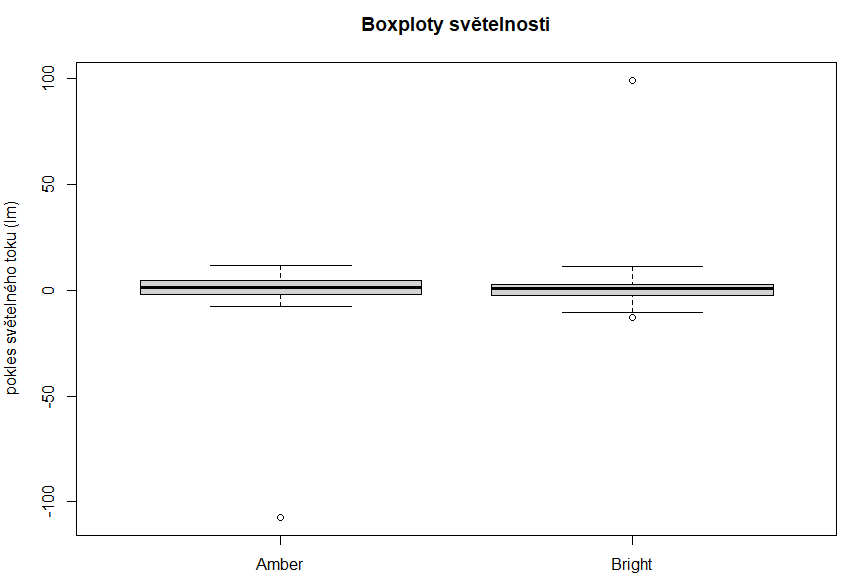
\includegraphics[width=0.9\textwidth]{Figures/Boxploty_2.png}
	\caption[Boxploty světelnosti, Amber a Bright]{Boxploty světelnosti, Amber a Bright}
	\label{fig:Boxplot2}
\end{figure}

U obou výrobců byly pozorovány 3 odlehlé pozorování (viz Obr. \ref{fig:Boxplot2}), tyto jsme se rozhodli z dálšího zpracování vypustit. 
Podle vizualizace srovnání poklesů světelného toku zářivek výrobců Amber a Bright (viz Obr. \ref{fig:Boxplot2}), Obr. \ref{fig:QQaHist})) lze usoudit, že k výraznému poklesu 
světelnéhu toku při snížení okolní teploty nedošlo.

\begin{figure}[H]
	\centering
	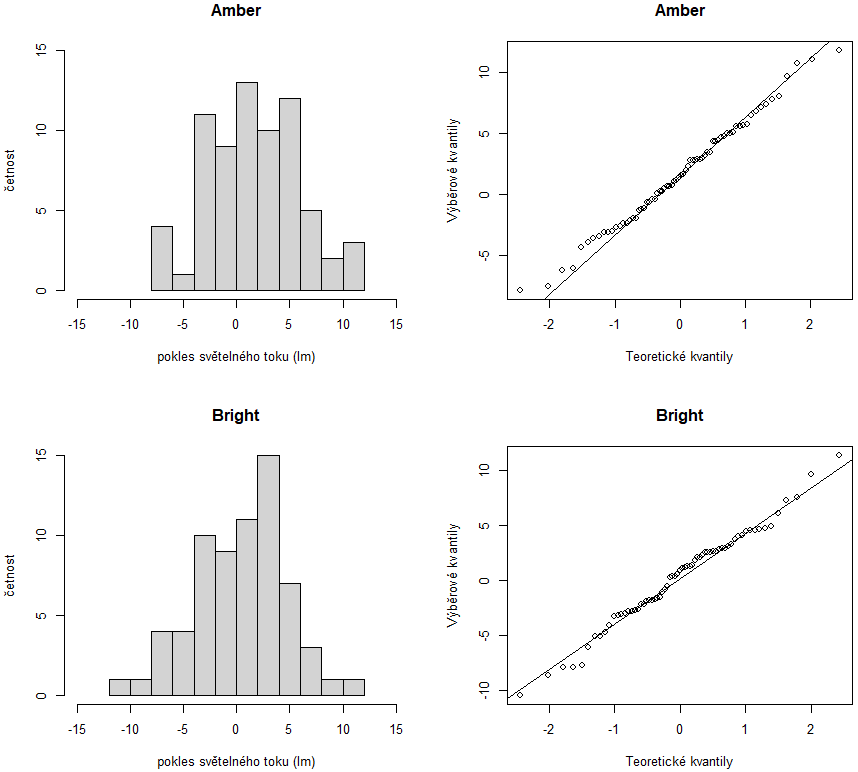
\includegraphics[width=0.9\textwidth]{Figures/QQaHistogram.png}
	\caption[Histogramy a Q-Q grafy světelnosti]{Histogramy a Q-Q grafy světelnosti, Amber a Bright, odstraněná pozorování}
	\label{fig:QQaHist}
\end{figure}


\newpage
\subsection{}
Na hladině významnosti 5 \% rozhodněte, zda jsou střední poklesy (popř. mediány poklesů) 
světelného tokuzářivek výrobců Amber a Bright statisticky významné. 
K řešení využijte bodové a intervalové odhady i testování hypotéz. Výsledky okomentujte.

Dle prezentovaných Q-Q grafů (viz Obr. \ref{fig:QQaHist}) lze usuzovat, že poklesy světelného toku zářivek u výrobce Amber i výrobce Bright 
lze modelovat normálním rozdělením. Šikmost i špičatost (viz Tab. \ref{tab:normSymet}) odpovídají normálnímu rozdělení.

\begin{table}[H]
	\centering
	\caption{Ověření normality poklesu světelného toku zářivek}
	\label{tab:normSymet}
    \begin{tabular}{c|c|c|c}
        & šikmost & stand. špičatost & \begin{tabular}[c]{@{}c@{}}Shapirův-Wilkův test\\ (p-hodnota)\end{tabular}  \\
        \hline
        výrobce Amber  & 0.12    & -0.35            & 0.87                                                         \\
        \hline
        výrobce Bright & -0.13   & 0.05             & 0.65                                                         \\
    \end{tabular}
\end{table}

Dle Shapirova-Wilkova testu lze na hladině významnosti 0,05 pokles světelného toku zářivek 
u výrobce Amber i u výrobe Bright modelovat normálním rozdělením (viz Tab. \ref{tab:normSymet}).

Rozdělení poklesů světelných toků zářivek lze u výrobce Amber i u výrobce Bright považovat za 
symetrické. (viz šikmosti, výsledky testu symetrie (Tab. \ref{tab:normSymet}) a tvar histogramů (Obr. \ref{fig:QQaHist})), 
proto lze pro intervalové odhady a test významnosti mediánu v případě obou výrobců použít Wilcoxonovu testovou statistiku.

Vzhledem k tomu, že očekáváme kladné poklesy kapacit (s klesající teplotou se 
světelný tok zářivek snižuje), volíme levostranné intervalové odhady / levostranné testy.

U zářivek výrobce Amber lze očekávat, že polovina bude vykazovat pokles světelného toku menší než cca 1.67 lm. 
95\% levostranný intervalový odhad mediánu poklesu světelného toku zářivek výrobce Amber je (14.9;$\infty$) lm.
Intervalový odhad, stejně jako p-hodnota Wilcoxonova testu, ukazují, že medián poklesu kapacit je statisticky významně větší než nula. 
Tj. na hladině významnosti 0,05 lze pokles světelného toku žárovek výrobce Amber považovat za statisticky významný (viz Tab. \ref{tab:medianWilc}). 

U zářivek výrobce Bright lze očekávat, že polovina bude vykazovat pokles světelného toku menší než cca 0.27 lm. 
95\% levostranný intervalový odhad mediánu poklesu světelného toku zářivek výrobce Bright je (14.3;$\infty$) lm.
Intervalový odhad, stejně jako p-hodnota Wilcoxonova testu, ukazují, že medián poklesu kapacit je statisticky významně větší než nula. 
Tj. na hladině významnosti 0,05 nelze pokles světelného toku žárovek výrobce Bright považovat za statisticky významný (viz Tab. \ref{tab:medianWilc}). 

\begin{table}[H]
	\centering
	\caption{Odhad mediánu a test významnosti poklesu světelných toků zářivek (lm) dle výrobce}
	\label{tab:medianWilc}
    \begin{tabular}{c|c|c|c}
        & \begin{tabular}[c]{@{}c@{}}bodový odhad\\ (lm)\end{tabular} & \begin{tabular}[c]{@{}c@{}}95\% levostranný\\ intervalový odhad\\ (lm)\end{tabular} & \begin{tabular}[c]{@{}c@{}}Studentů \\ levostranný t-test\\ (p-hodnota)\end{tabular} \\
        \hline
        výrobce Amber  & 1.67                                                        & 14.9                                                                                & \textless{}0.001                                                     \\
        \hline
        výrobce Bright & 0.27                                                        & 14.3                                                                                & 0.31                                                                 \\
    \end{tabular}
\end{table}


\newpage
\subsection{}
Na hladině významnosti 5\% rozhodněte, zda je rozdíl středních hodnot (mediánů) 
poklesů světelných toků zářivek výrobců Amber a Bright (při snížení okolní teploty) statisticky významný.
K řešení využijte bodový a intervalový odhad i čistý test významnosti. Výsledky okomentujte.

Vzhledem k potvrzení normality u výrobce Amber i Bright je třeba zjistit zda mezi rozptyly výrobců panuje shoda.

Na základě výsledku F-testu (viz Tab. \ref{tab:medianStudent}) lze rozhodnout o shodě rozptylů (homoskedasticitě) a použít 
Dvouvýběrový Studentův t-test pro test stř. hodnot.

U zářivek výrobce Amber lze očekávat pokles ve světelném toku o cca 1.4 lm větší než u výrobce Bright. 
Odpovídající 95\% levostranný intervalový odhad tohoto rozdílu je (0.69;$\infty$) lm.
Intervalový odhad, stejně jako Dvouvýběrový Studentův t-test (viz Tab. \ref{tab:medianStudent}) ukazují, že medián 
poklesu světelného toku zářivek výrobce Amber není statistiky významně vyšší než u výrobce Bright.

\begin{table}[H]
	\centering
	\caption{Srovnání mediánu poklesu světelných toků zářivek (lm) výrobce Amber a Bright}
	\label{tab:medianStudent}
    \begin{tabular}{c|c}
        Bodový odhad $X_{0.5}^A$ - $X_{0.5}^B$ (lm)                                   & 1.40        \\
        \hline
        F-test (p-hodnota)                                                    & 0.44        \\
        \hline
        95\% levostranný intervalový odhad $X_{0.5}^A$ - $X_{0.5}^B$ (lm)     & (0.69;$\infty$)  \\
        \hline
        Dvouvýběrový Studentův t-test (p-hodnota)                             & 0.5         \\
    \end{tabular}
\end{table}

\end{document}

